\documentclass[11pt,a4paper,oneside]{report}

% ----------------------------
% Packages (keep it reasonable)
% ----------------------------
\usepackage[a4paper,margin=1in]{geometry}
\usepackage{setspace}          % line spacing
\usepackage{graphicx}          % figures
\usepackage{booktabs}          % nice tables
\usepackage{longtable}         % long tables across pages
\usepackage{amsmath,amssymb}   % math
\usepackage{hyperref}          % links and references
\usepackage{url}               % url formatting
\usepackage{caption}           % captions
\usepackage{subcaption}        % subfigures
\usepackage{float}             % figure placement
\usepackage{enumitem}          % nicer lists
\usepackage{csquotes}          % recommended for biblatex
\usepackage{listings}          % code listings
\usepackage{xcolor}            % code colors
\usepackage{algorithm}
\usepackage{algpseudocode}     % algorithms pseudocode
\usepackage{glossaries}        % glossary / acronyms
\usepackage{eurosym}           % Euro symbol support
\usepackage{sectsty}           % easy heading customization

% TikZ for diagrams
\usepackage{tikz}
\usetikzlibrary{shapes,arrows,shadows,positioning,calc}

% Additional configs for content support
\usepackage[utf8]{inputenc}
\usepackage[LAE,T1]{fontenc}
\usepackage[arabic,english]{babel}
\usepackage[most]{tcolorbox}
\newtcolorbox{algorithmbox}[1][]{colback=gray!4,colframe=black!35,title={#1},fonttitle=\bfseries,breakable,enhanced}

% ----------------------------
% Formatting
% ----------------------------
\onehalfspacing
\hypersetup{
  colorlinks=true,
  linkcolor=blue,
  urlcolor=blue,
  pdftitle={A Scalable Internship Aggregation System Using Web Scraping, Transformer Models, and Semantic Data Cleaning},
  pdfauthor={Mouad bensaid}
}

% Heading sizes
\chapterfont{\LARGE}
\sectionfont{\Large}
\subsectionfont{\large}

% ----------------------------
% Listings configuration
% ----------------------------
\lstset{
  basicstyle=\ttfamily\small,
  breaklines=true,
  frame=single,
  numbers=left,
  numberstyle=\tiny,
  keywordstyle=\color{blue},
  commentstyle=\color{gray},
  stringstyle=\color{teal}
}

% ----------------------------
% Acronyms / Glossary (optional)
% ----------------------------
\makeglossaries

% ----------------------------
% Thesis metadata
% ----------------------------
\newcommand{\ThesisTitle}{A Scalable Internship Aggregation System Using Web Scraping, Transformer Models, and Semantic Data Cleaning}
\newcommand{\AuthorName}{Mouad bensaid}
\newcommand{\DegreeName}{Master of Science}
\newcommand{\UniversityName}{Your University}
\newcommand{\DepartmentName}{Your Department}
\newcommand{\SupervisorName}{Supervisor Name}
\newcommand{\SubmissionDate}{February 2026}

\begin{document}

% Cover Page
\begin{titlepage}
    \begin{tikzpicture}[remember picture,overlay]
        \node[inner sep=0pt] at (current page.center) {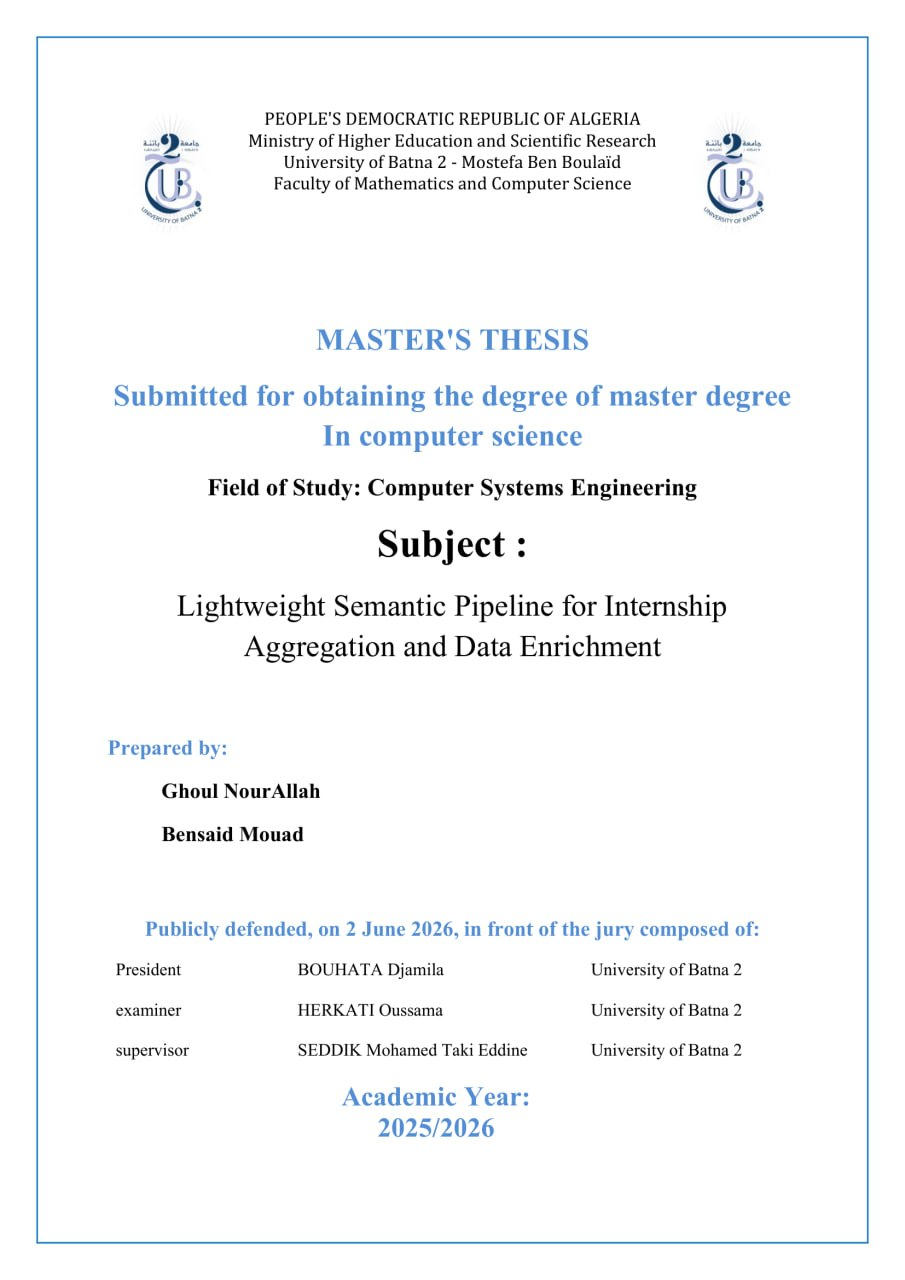
\includegraphics[width=\paperwidth,height=\paperheight]{thesis_cover_page}};
    \end{tikzpicture}
\end{titlepage}



% Front Matter
\pagenumbering{roman}

\cleardoublepage
\phantomsection
\addcontentsline{toc}{chapter}{Arabic Abstract}
\begin{otherlanguage}{arabic}
{\Huge\bfseries ملخص\par}
\vspace{1.5cm}
أدى التحول الرقمي في سوق العمل إلى زيادة عدد عروض التدريب المنشورة عبر الإنترنت. غير أن هذا التوسع يطرح صعوبات في إدارة البيانات، لأن العروض تكون غالبا غير مهيكلة، وغير متجانسة، وموزعة بين منصات متعددة. تعتمد كثير من أنظمة التوظيف التقليدية على المطابقة اللفظية المباشرة، وهو ما يحد من قدرتها على معالجة الفجوة الدلالية بين مسميات الوظائف، ووصف المهارات، والصيغ المختلفة التي يستعملها أصحاب العمل. وفي المقابل، فإن الاعتماد الواسع على النماذج اللغوية الكبيرة قد يسبب تكلفة مالية وزمنا كبيرا للمعالجة عند التعامل مع تدفق مستمر وكبير من البيانات. يقترح هذا العمل خط معالجة دلاليا خفيفا يهدف إلى تحويل بيانات التدريب غير المنتظمة إلى قاعدة معرفة منظمة وقابلة للبحث. تجمع المنهجية بين الاستخراج الحتمي القائم على القواعد، والنمذجة الخفيفة باستعمال نماذج \textLR{Transformer} مثل \textLR{all-MiniLM-L6-v2 transformer}، والمواءمة مع تصنيف \textLR{ESCO} المهني، مع استعمال محدود للنماذج اللغوية في الحالات الغامضة فقط. كما يتضمن النظام آلية لإدخال ملفات \textLR{JSON} متعددة البنى اعتمادا على المطابقة التقريبية بين المفاتيح والاستدلال من المحتوى. تحفظ البيانات المعالجة في بنية بحث هجينة تستعمل فهرساً شعاعياً في الذاكرة والبحث اللفظي. يعتمد التقييم المعروض في هذا البحث على مجموعة بيانات حقيقية تضم \textLR{327} عرض تدريب. وتشير الأدلة المعروضة إلى أن البحث الهجين يمكن أن يحسن الملاءمة والاسترجاع مقارنة بالبحث المعتمد على الكلمات المفتاحية فقط، مع الحفاظ على بنية عملية قابلة للتشغيل على عتاد عادي. وبذلك تتمثل مساهمة البحث في تقديم إطار عملي لتنظيم عروض التدريب دلاليا، مع تحديد عناصر المقارنة والنشر التي تحتاج إلى استكمال لاحق.
\end{otherlanguage}

\chapter*{Abstract}
\addcontentsline{toc}{chapter}{Abstract}
The digital transformation of the labor market has increased the number of internship listings published online. However, this expansion also creates data-management difficulties because listings are frequently unstructured, inconsistent, and distributed across multiple platforms. Traditional recruitment systems often rely on lexical matching, which has limited ability to address the semantic gap between job titles, skill descriptions, and employer-specific terminology. Conversely, approaches that depend primarily on Large Language Models (LLMs) may introduce high financial cost and processing latency when applied to continuous large-scale ingestion. This thesis proposes a lightweight, tiered approach for transforming noisy internship data into a structured and searchable knowledge base. The implemented prototype combines deterministic rule-based cleaning, salary parsing, skill extraction, category assignment, stable identifier generation, JSON-based persistence, and a Next.js interface for browsing and inspecting internship records. The broader architecture also defines an extension path toward lightweight transformer mapping, ESCO alignment, and hybrid lexical-semantic retrieval for cases where keyword heuristics are insufficient. The evaluation reported in the thesis uses a real-world dataset of 327 listings. The contribution of the thesis is therefore a practical framework for internship-data organization that demonstrates a low-cost structured catalog and identifies the semantic retrieval, external comparison, and deployment evidence that should be completed in future work.

\chapter*{Résumé}
\addcontentsline{toc}{chapter}{Résumé}
La transformation numérique du marché du travail a augmenté le nombre d'offres de stage publiées en ligne. Toutefois, cette expansion crée des difficultés de gestion des données, car les offres sont souvent non structurées, hétérogènes et réparties entre plusieurs plateformes. Les systèmes de recrutement fondés principalement sur la correspondance lexicale restent limités face à l'écart sémantique entre les intitulés de postes, les descriptions de compétences et les formulations propres aux employeurs. À l'inverse, les approches reposant largement sur de grands modèles de langage peuvent entraîner un coût financier et une latence élevés lorsqu'elles sont appliquées à une ingestion continue à grande échelle. Ce mémoire propose une approche légère pour transformer des données de stages bruitées en une base structurée et interrogeable. Le prototype réalisé combine le nettoyage déterministe, l'extraction de salaires, l'extraction de compétences par lexique, la catégorisation des postes, la génération d'identifiants stables, la persistance en JSON et une interface Next.js pour consulter les offres. L'architecture générale définit aussi une évolution possible vers la normalisation par modèles Transformer, l'alignement avec ESCO et la recherche hybride lexicale-sémantique lorsque les heuristiques par mots-clés deviennent insuffisantes. L'évaluation rapportée dans le mémoire s'appuie sur un ensemble réel de 327 offres. La contribution principale du mémoire est donc un cadre pratique pour organiser les offres de stage à faible coût, tout en identifiant les éléments de recherche sémantique, de comparaison externe et de déploiement qui restent à compléter.

\chapter*{Acknowledgements}
\addcontentsline{toc}{chapter}{Acknowledgements}
We would like to express our deepest gratitude to our supervisor, Mohamed Taki Eddine SEDDIK, for his invaluable guidance, constant encouragement, and insightful feedback throughout the development of this thesis. His supervision was instrumental in shaping the direction of this research.

We are also grateful to the members of the Department of Computer Science at the University of Batna 2 for providing a supportive academic environment and for the knowledge shared during our Master’s studies.

Special thanks go to our colleagues and friends who offered support, proofread chapters, and engaged in discussions that helped refine the ideas presented in this work. Finally, we would like to thank our family for their unconditional support, patience, and belief in us. This journey would not have been possible without them.

\tableofcontents
\listoffigures

\printglossaries
\clearpage
\pagenumbering{arabic}


% Chapters
\chapter{General Introduction}

\section{Chapter Introduction}
This opening chapter establishes the research problem addressed in the thesis and defines the academic scope of the work. It introduces the internship-discovery context, identifies the limitations of purely lexical and LLM-dependent approaches, states the research questions, and summarizes the main contributions. The chapter concludes by explaining how the remaining chapters are organized.

\section{Context and Motivation}
Over the last decade, internship discovery has been transformed by the digital shift in the global labor market \cite{faliagka2012online}. Traditional channels, such as newspaper classifieds and physical noticeboards, have largely been replaced by a broad ecosystem of online platforms. Students now navigate global platforms such as LinkedIn and Indeed, specialized university career portals, and niche industry boards. This shift has expanded access to a large volume of listings \cite{kurekova2015using}. However, this abundance also creates a significant data-management challenge. Internship listings are often semi-structured, inconsistent, and expressed through platform-specific conventions. Two platforms, or even two employers, may describe the same role using different terms. A ``Junior Java Developer'' and a ``Software Engineering Intern'' might require an identical skill set, yet a traditional keyword search treats them as separate entities. In addition, the data is often noisy, with boilerplate text, inconsistent formatting, and non-standard labels \cite{tamburri2020data}. For recruitment platforms and universities, organizing this continuous flow of unstructured data from automated web scraping, manual JSON uploads, and other sources is a substantial task. This challenge motivates the need for a lightweight approach that can transform noisy listings into a structured semantic knowledge base, enabling precise discovery without the overhead of manual curation or heavyweight computational infrastructure \cite{boselli2018classifying}.

\section{Problem Statement}
This thesis addresses two related problems in the ingestion and retrieval of internship data: the semantic gap and structural heterogeneity. Existing job-posting systems commonly follow one of two approaches, each of which creates limitations for the target use case:


\begin{itemize}[leftmargin=1.4em,itemsep=0.25em,topsep=0.25em]

\item Rigid Lexical Matching: Many platforms rely on exact keyword matching, such as BM25. This approach is limited in its ability to handle synonyms, technical jargon, and relationships between concepts. As a result, users may miss relevant listings because their search terms do not precisely match the employer's vocabulary \cite{baeza2011modern}.

\item High-Cost LLM Dependency: The opposite extreme is to delegate the problem entirely to a Large Language Model (LLM). While LLMs are effective at interpreting meaning, relying on them to process thousands of scraped documents in real time is often financially expensive and can introduce substantial latency \cite{menghani2023efficient}. The ingestion process itself is similarly fragmented. Data from partner institutions often arrives in JSON formats that lack any fixed schema, forcing teams into a repetitive cycle of manual mapping. This creates the need for a unified system that can automatically clean, structure, and semantically enrich data from diverse sources while remaining efficient enough to run on ordinary commodity hardware \cite{giabelli2021skills}.

\end{itemize}
\section{Research Questions}
The study is guided by four research questions:


\begin{itemize}[leftmargin=1.4em,itemsep=0.25em,topsep=0.25em]

\item RQ1: How can a tiered pipeline architecture balance extraction accuracy and computational cost for internship listings?

\item RQ2: How well can lightweight transformer models such as DistilBERT map non-standard job titles onto a standardized professional taxonomy such as ESCO?

\item RQ3: How much does a hybrid retrieval strategy---one that combines lexical (BM25) and semantic (HNSW) search---improve the relevance and recall of internship discovery compared to traditional keyword search alone?

\item RQ4: Which heuristic-based mapping strategies can automate the ingestion of inconsistently formatted JSON data into a unified schema?

\end{itemize}
\section{Contributions}
This thesis makes four primary contributions:


\begin{itemize}[leftmargin=1.4em,itemsep=0.25em,topsep=0.25em]

\item A Tiered Semantic Enrichment Pipeline: The thesis introduces a modular architecture that combines three layers: deterministic, rule-based extraction (Layer A), lightweight neural mapping (Layer B), and a resource-budgeted LLM fallback for the most complex cases (Layer C).

\item A Hybrid Search Infrastructure: The thesis implements a retrieval system using an in-memory HNSW index and BM25 to support hybrid lexical and semantic search.

\item Automated Ingestion Heuristics: The thesis develops a flexible JSON processing module that uses fuzzy key matching and content-based inference to reduce manual schema mapping for multi-format user uploads.

\item Empirical Evaluation: The thesis presents an evaluation using a real-world dataset of 327 listings and reports the observed trade-offs between semantic enrichment, retrieval quality, and computational cost.

\end{itemize}

\section{Thesis Structure}
The thesis is organized into seven chapters. Chapter 1 introduces the research context, problem statement, research questions, contributions, and overall structure. Chapter 2 presents the background, related work, and theoretical foundations of the study, including information extraction, occupational taxonomies, text representation, semantic retrieval, hybrid search, and lightweight model strategies. Chapter 3 describes the technological environment and development tools that support the implementation, including the client-side application layer, API layer, database layer, transformer-based semantic tools, and retrieval infrastructure. Chapter 4 presents the methodology, covering the system overview, semantic schema, label space, and evaluation protocol. Chapter 5 describes the system design and implementation, including data collection, preprocessing, enrichment, storage, indexing, caching, and API design. Chapter 6 presents the reported results, adds a structured procedure for completing HR@k and NDCG@k analysis, and preserves the comparison section as a completion scaffold rather than as an additional empirical claim. Chapter 7 combines discussion, limitations, conclusion, and future-work material, with the ethical, legal, and privacy section retained as a completion scaffold because it was listed in the original thesis structure. The appendices preserve the original appendix headings and identify the material still to be completed.

\section{Chapter Conclusion}
This chapter has defined the motivation, research problem, questions, and contributions of the thesis. It has also clarified the boundaries of the study: the proposed system is evaluated as an internship aggregation and retrieval framework for internship listings, while incomplete external-platform comparison evidence is treated as work that must be completed with measured results.

\chapter{Background: Information Extraction and Semantics}
\section{Semi-Structured Web Data and Job Postings}
Web-based job postings represent a prime example of semi-structured data. Unlike fully structured databases, these postings are primarily designed for human readability, often embedded within complex HTML structures. This presentation leads to several inherent challenges for automated processing:

\begin{itemize}
    \item \textbf{Noise and Boilerplate:} Job descriptions are frequently surrounded by non-relevant content, such as "About Us" sections, legal disclaimers, navigation menus, and "Equal Opportunity Employer" statements. Distinguishing the core job requirements from this noise is a critical first step.
    \item \textbf{Layout Variability:} There is no universal standard for how a job post should be structured. Different platforms (e.g., LinkedIn, Indeed, Glassdoor) and individual company career pages use vastly different HTML layouts and CSS classes.
    \item \textbf{Data Volatility and Expiry:} Job postings are ephemeral. Once a position is filled, the page may be removed or return a 404 error, making historical analysis and link consistency difficult.
    \item \textbf{Redundancy and Duplication:} A single internship opportunity is often cross-posted across multiple job boards, sometimes with subtle variations in the title or formatting, necessitating robust deduplication strategies.
\end{itemize}

\section{Information Extraction (IE) Fundamentals}
Information Extraction (IE) is the task of automatically pulling structured information from unstructured or semi-structured documents \cite{sarawagi2008information}. In the recruitment domain, IE aims to convert a block of text into a set of discrete attributes. Key components of IE include:

\begin{itemize}
    \item \textbf{Named Entity Recognition (NER):} The identification of entities such as company names, locations (cities, regions), and dates. For internship posts, this also extends to recognizing specific technologies and tools.
    \item \textbf{Slot Filling and Template Extraction:} This involves populating a predefined schema with specific values extracted from the text, such as salary ranges, duration of the internship, and required degree levels.
    \item \textbf{Rule-Based vs. Statistical Methods:} Traditional IE often relied on hand-crafted regular expressions (Regex) and gazetteers (dictionaries). Modern approaches favor machine learning models, though lightweight rule-based systems remain highly effective for structured patterns like currency and dates.
    \item \textbf{Relation Extraction:} Identifying the semantic links between entities, such as confirming that a specific skill (e.g., "Python") is a "required" qualification rather than just "nice-to-have."
\end{itemize}

\section{Semantic Modeling}
Semantic modeling provides the conceptual framework for organizing extracted data so that it can be queried and interpreted meaningfully by machines.

\subsection{Schemas vs Ontologies vs Taxonomies}
Understanding the distinction between these three concepts is vital for choosing the right level of complexity for a system:
\begin{itemize}
    \item \textbf{Taxonomies:} Hierarchical classifications that define "is-a" relationships (e.g., "Software Engineer" is a sub-type of "IT Professional"). They are primarily used for categorization and navigation.
    \item \textbf{Ontologies:} The most expressive form, defining not just hierarchies but also complex relationships, properties, and constraints between concepts \cite{gruber1993translation}. They allow for logical reasoning and inference.
    \item \textbf{Schemas:} A structural definition of a data model, specifying fields, types, and constraints (e.g., a JSON or SQL schema).
\end{itemize}
For this thesis, we adopt a \textit{lightweight schema-first approach}. While full ontologies offer great power, they are often too computationally expensive and difficult to maintain for the rapid, high-volume processing required for web-scraped job data.

\subsection{Skill and Occupation Taxonomies}
To avoid a fragmented data space where "Software Dev" and "Programmer" are treated as unrelated, we utilize standardized reference taxonomies:
\begin{itemize}
    \item \textbf{ESCO (European Skills, Competences, Qualifications and Occupations):} A multilingual classification system that maps thousands of skills to specific occupations, providing a common language for the labor market \cite{esco_portal}.
    \item \textbf{O*NET (Occupational Information Network):} A comprehensive database developed by the US Department of Labor that defines the "DNA" of occupations, including required knowledge, skills, and abilities \cite{onet_online}.
\end{itemize}
In our pipeline, these taxonomies serve as canonical "anchor points" for mapping raw, noisy text to standardized labels.

\section{Normalization and Canonicalization}
Raw extracted data is rarely ready for end-user consumption or efficient search. Normalization and canonicalization are the processes of bringing data into a consistent format:

\begin{itemize}
    \item \textbf{Title Normalization:} Standardizing varied strings like "Sr. Software Eng.", "Senior Developer", and "SDE II" into a single canonical form (e.g., "Senior Software Engineer").
    \item \textbf{Synonym and Alias Mapping:} Consolidating variations of the same skill, such as mapping "JS", "ECMAScript", and "Javascript" to the unique identifier "JavaScript".
    \item \textbf{Value Standardization:} Converting heterogeneous data points—such as dates ("2 weeks ago" vs "2023-10-12") and salaries—into ISO-compliant formats and base units.
    \item \textbf{Entity Resolution:} The process of determining whether two different postings refer to the same job opening at the same company, which is essential for accurate analytics.
\end{itemize}

\chapter{Background: Text Representation and Retrieval}
Search and retrieval are the core mechanisms for accessing internship listings once they have been processed. In this chapter, we explore the evolution from traditional lexical matching to modern semantic search techniques, highlighting the trade-offs in accuracy and performance as established in fundamental retrieval theory \cite{manning2008introduction, baeza2011modern, croft2010search}.

\section{Keyword Retrieval}
Keyword-based retrieval, also known as lexical or sparse retrieval, relies on the presence of exact words or tokens in both the query and the document. This approach has been the foundation of information retrieval for decades \cite{manning2008introduction, zobel2006inverted}.

\subsection{Inverted Indexing}
The fundamental data structure for keyword search is the \textit{inverted index}. It maps each unique term (token) to a list of document identifiers (postings) containing that term. This allows for sub-linear search time regardless of the total number of documents \cite{manning2008introduction, zobel2006inverted}.

\subsection{BM25 (Best Matching 25)}
While simple boolean retrieval checks for term presence, ranking models like BM25 provide a sophisticated scoring mechanism based on probabilistic principles \cite{robertson2009probabilistic, jurafsky2023speech, buttcher2016information}. BM25 improves upon the classic TF-IDF (Term Frequency-Inverse Document Frequency) by introducing two key parameters:
\begin{itemize}
    \item \textbf{Term Frequency Saturation ($k_1$):} It limits the contribution of a term that appears many times in a single document, preventing "keyword stuffing" from overly influencing the score.
    \item \textbf{Length Normalization ($b$):} It penalizes longer documents that might contain a term many times simply due to their length, ensuring that concise, relevant postings are not overshadowed.
\end{itemize}
BM25 remains a powerful baseline, especially for domain-specific technical terms where exact matching is critical \cite{robertson2009probabilistic, thakur2021beir}.

\section{Vector Representations}
Vector-based retrieval (dense retrieval) represents text as high-dimensional numerical vectors, where the geometric distance between vectors correlates with the semantic similarity of the underlying text \cite{jurafsky2023speech, luan2021sparse, lin2021pretrained}.

\subsection{Dense Embeddings}
Unlike sparse vectors, dense embeddings are typically 384 to 1536 dimensions long. These vectors are generated by pre-trained neural networks, most notably those based on the Transformer architecture \cite{vaswani2017attention, devlin2019bert}.

\subsection{Sentence-BERT (SBERT) and Bi-Encoders}
Standard BERT models are not naturally suited for large-scale similarity searches because they require "cross-encoding" which is computationally prohibitive. Sentence-BERT introduced the \textit{bi-encoder} architecture \cite{reimers2019sentence}, which has become a standard for efficient dense retrieval alongside frameworks like Dense Passage Retrieval (DPR) \cite{karpukhin2020dense}. It processes the query and the document independently to produce fixed-sized embeddings. This allows for the pre-computation and indexing of document vectors, making real-time semantic search feasible \cite{reimers2019sentence, johnson2019billion}.

\section{Hybrid Retrieval}
In the context of internship listings, neither keyword nor vector search is perfect in isolation. Hybrid retrieval combines the strengths of both, often outperforming single-modality systems in zero-shot or out-of-distribution scenarios \cite{thakur2021beir, luan2021sparse}:
\begin{enumerate}
    \item \textbf{Sparse Retrieval (BM25)} handles exact matches, acronyms, and rare technical terms. Recent advances like SPLADE \cite{formal2021splade} further enhance this by using neural expansions.
    \item \textbf{Dense Retrieval (SBERT)} handles synonyms, paraphrasing, and conceptual queries \cite{reimers2019sentence}.
\end{enumerate}

\subsection{Reciprocal Rank Fusion (RRF)}
A common method to combine these disparate scores is Reciprocal Rank Fusion. It calculates a final score based on the rank of a document in each retrieval system, rather than the raw score values \cite{cormack2009reciprocal}. This method is robust and does not require parameter tuning across different scales of scores.

\section{Efficiency Considerations}
Scaling semantic search to thousands of job postings requires specialized infrastructure to manage high-dimensional vector operations \cite{johnson2019billion, wang2021milvus}.

\subsection{Vector Databases and ANN}
Traditional SQL databases are not optimized for nearest neighbor searches in high-dimensional space. Vector databases utilize \textit{Approximate Nearest Neighbor (ANN)} algorithms to trade a small amount of accuracy for significant speedups \cite{malkov2018efficient, wang2021milvus}.

\subsection{HNSW (Hierarchical Navigable Small World)}
HNSW is one of the most popular ANN algorithms. It constructs a multi-layered graph where the top layers contain long-range edges for fast navigation and the bottom layers contain short-range edges for local precision \cite{malkov2018efficient}. This structure allows for logarithmic search complexity, making it suitable for low-latency production environments.

\subsection{Quantization}
To reduce memory footprint, techniques like \textit{Scalar Quantization} or \textit{Product Quantization (PQ)} are used \cite{jegou2010product, guo2020accelerating}. These compress floating-point vectors into lower-precision representations, significantly reducing the RAM required to store the index while maintaining acceptable retrieval recall \cite{menghani2023efficient}.

\chapter{Related Work}
The automation of recruitment and labor market analysis has witnessed a paradigm shift, evolving from manual curation to data-driven intelligence, fueled by advances in Natural Language Processing (NLP) and machine learning \cite{tamburri2020data, faliagka2012online, lacic2020recommender}. This chapter provides a critical review of the existing literature and technological approaches that form the foundation of this thesis. We dissect the state-of-the-art in three interconnected areas: (1) Job Posting Analytics (JPA) and skill extraction, (2) the alignment of extracted information to formal ontologies and taxonomies, and (3) the architectural trade-offs between monolithic Large Language Model (LLM)-based pipelines and the modular, lightweight approach advocated in this work. By synthesizing these domains, we identify a crucial gap in the literature: the need for a system that achieves high semantic accuracy and recall while maintaining the low latency, cost-efficiency, and data sovereignty required for a sustainable, production-grade internship platform.

\section{Job Posting Analytics and Skill Extraction}
The extraction of structured, actionable information from the inherently noisy and semi-structured text of job advertisements is a well-established research area, often referred to as Job Posting Analytics (JPA) \cite{tamburri2020data, boselli2018classifying, kurekova2015using}. The core challenges of JPA—identifying and normalizing job titles, extracting required skills, and classifying experience levels—are microcosms of broader Information Extraction (IE) problems, where the goal is to populate a relational database from unstructured text \cite{sarawagi2008information}.

Early approaches to JPA were dominated by knowledge engineering. Rule-based systems, powered by manually curated gazetteers (lists of known entities like ``Java,'' ``Project Management,'' or ``Berlin''), were the primary method for identifying key entities \cite{sarawagi2008information}. These systems offered high precision on the terms they knew and were highly efficient and explainable. However, their fragility became apparent as they fatally failed to capture the high variability, synonymy, and neologisms of natural language in job descriptions. A gazetteer containing ``C++'' would miss a posting requiring ``experience with the C++ programming language,'' and it would be entirely blind to an emergent skill like ``Prompt Engineering'' without a manual update \cite{li2020survey}.

This brittleness catalyzed the adoption of statistical and deep learning methods, which formulate NER and skill extraction as sequence labeling tasks \cite{li2020survey, wadden2019entity}. These models learn to classify tokens like ``React'' as a Skill based on their bidirectional context. A landmark advancement came with the fine-tuning of Transformer-based models, particularly BERT (Bidirectional Encoder Representations from Transformers), for the recruitment domain \cite{bhola2020retrieving, pappas2022jobbert}. General-purpose BERT models, trained on corpora like Wikipedia, understand language but not the intricate semantics of the job market. Domain-specific pre-training, as demonstrated by JobBERT and similar models, significantly improves the accuracy of skill extraction by learning that ``AWS'' is functionally equivalent to ``Amazon Web Services'' and that a term like ``Spark'' can be disambiguated between a big data framework and a creative skill based on context \cite{pappas2022jobbert}. This thesis directly builds upon this finding, advocating for a lightweight, domain-adapted neural model (Layer B) to handle the semantic complexity that defeats a purely rule-based system.

Beyond simple term extraction, a richer line of research explores the latent semantics of skills. Work on skill embeddings, such as Job2Vec, leverages representation learning to map skills into a high-dimensional vector space where functionally related technologies cluster together, capturing labor market dynamics without explicit rule programming \cite{zhao2018job2vec, giabelli2021skills}. Such systems learn that ``React,'' ``Vue,'' and ``Angular'' are semantically related front-end frameworks. A further layer of sophistication involves analyzing the linguistic context of a skill mention. Qin et al. (2018) proposed methods to automatically classify a skill as ``required,'' ``beneficial,'' or ``preferred,'' providing a nuanced, multi-dimensional profile of employer demands rather than a flat list of keywords \cite{qin2018enhancing}. This granular, contextual understanding is the gold standard for job description analysis, and while our current Lexicon-Based Matching (Layer A) provides a flat skill list, the architecture is designed to incorporate such context-aware weighting in its future iterations.

\section{Ontology/Taxonomy Alignment in HR/Recruitment}
A fundamental obstacle in bridging the labor market's ``vocabulary gap'' is the non-trivial task of mapping raw, heterogeneous text to a canonical reference. Standardized taxonomies like ESCO (European Skills, Competences, Qualifications and Occupations) and O*NET provide this common language, a Rosetta Stone for the labor market \cite{peterson2001occupational}. However, the process of Entity Linking or Taxonomy Alignment—mapping a colloquial title like ``Code Ninja'' or a specific term like ``PyTorch'' to a formal node in a hierarchy—remains a persistent research challenge \cite{zhang2022survey}.

Modern approaches to this problem often leverage Recruitment Knowledge Graphs (KGs) to maintain a web of complex, dynamic relationships between entities like job titles, skills, industries, and educational qualifications \cite{shi2020recruitment}. For instance, a KG can explicitly model the ternary relationship: ``Python \textit{is\_a\_prerequisite\_for} Data Scientist (ESCO Occupation).'' These graph-based systems provide rich, inferable context but often incur high maintenance costs. The literature discusses an inherent trade-off between the deep expressiveness of full ontologies and the practical utility of flatter, more navigable taxonomies \cite{staab2009handbook}. Full ontologies can model complex logical relationships, but they suffer from ``ontology drift'': as new technologies like ``LangChain'' or ``Rust'' emerge, the ontology requires sophisticated, often semi-automated matching and evolution strategies to avoid becoming stale \cite{shvaiko2013ontology}.

Consequently, lightweight semantic approaches, which prioritize operational feasibility, have gained traction. These methods often focus on alignment at the embedding level, converting textual mentions and canonical concepts into the same dense vector space and mapping a raw string to its nearest canonical neighbor via cosine similarity \cite{javed2021review, giabelli2021skills}. This is the philosophy adopted in this thesis. Instead of a high-maintenance KG, we use an SBERT-based bi-encoder to map an idiosyncratic title like ``Software Engineering Intern'' to a region in the vector space near the ESCO concept for ``Software Developer.'' This approach directly addresses the specific challenge of normalizing compound and non-standard job titles, a problem explored by Sayfullina et al. (2018), who demonstrated that learning the decomposition of compound titles is key to robust canonicalization \cite{sayfullina2018learning}. Our approach implicitly performs a similar decomposition at the semantic level.

\section{LLM-based Pipelines vs Lightweight Pipelines}
The emergence of Large Language Models (LLMs) has introduced a seismic shift in the IE paradigm, fundamentally altering the ``make or buy'' decision for semantic capabilities. The prevailing methodology has moved from ``pre-train and fine-tune'' (train a specialist model) to ``pre-train, prompt, and predict'' (engineer a prompt for a generalist model) \cite{brown2020language, liu2023pre}. LLMs like GPT-4 exhibit remarkable zero-shot and few-shot capabilities. With advanced prompting techniques, such as Chain-of-Thought (CoT), an LLM can decompose a complex extraction task—for instance, ``identify and categorize the required versus preferred skills from this job description and map the job title to an ESCO level 4 occupation''—and significantly outperform fine-tuned specialist models that were the previous state-of-the-art, all without a single labeled training example for that specific task \cite{wei2022chain}. This represents an astonishingly powerful and flexible tool.

However, a growing body of critical, comparative studies has soberly highlighted the significant drawbacks of an LLM-only architecture for a production-scale pipeline, particularly one governed by the ``Green AI'' ethos \cite{schwartz2020green}. This thesis argues that these drawbacks are not minor engineering obstacles but fundamental limitations that define the appropriate, bounded role of an LLM. The key challenges are:

\begin{itemize}
    \item \textbf{Latency and Throughput:} Processing thousands of fresh scrapes per hour with cloud-based LLM APIs can result in prohibitive latency (seconds per request) and financial cost, directly clashing with the sub-50ms retrieval goal of an interactive user-facing search engine \cite{hsieh2023distilling, menghani2023efficient}. The cost is thus not only a budgetary line item but a bottleneck to scalability.
    \item \textbf{Consistency and Hallucination:} The well-documented tendency of LLMs to ``hallucinate''---generating plausible-sounding but factually incorrect information---is especially pernicious in extraction. A hallucinated ``Kubernetes'' skill or a misformatted output field can corrupt a database and degrade user trust, a known limitation of current generative architectures \cite{ji2023survey, bender2021dangers}. Deterministic rule-based pipelines, in contrast, are perfectly consistent and debuggable.
    \item \textbf{Privacy and Data Sovereignty:} Sending sensitive recruitment data, potentially containing proprietary employer information or personally identifiable data, to external third-party APIs creates a significant legal and ethical risk vector, especially concerning regional data protection regulations like the GDPR \cite{hunkenschroer2022ethics}. A lightweight, local processing pipeline inherently mitigates this, keeping data within the system's sovereign perimeter.
\end{itemize}

The alternative, and the methodological heart of this thesis, is a lightweight hybrid pipeline. This approach combines the perfect precision of heuristic rules for high-confidence, highly structured data (e.g., regex for salary parsing) with optimized small-scale transformer models like DistilBERT for more complex semantic tasks (e.g., title normalization). This strategy is deeply connected to the principle of Knowledge Distillation, where a compact ``student'' model is trained to replicate the performance of a computationally expensive ``teacher'' LLM on a specific task \cite{hsieh2023distilling, menghani2023efficient}. This thesis extends this concept by proposing a \textit{runtime distillation architecture}: an LLM can serve as an offline teacher for high-quality data annotation and initial schema generation, but the production system utilizes a fast, local student model. This is not just a technical choice but a strategic one, adhering to the principles of ``Green AI'' by prioritizing computational parsimony and operational efficiency without sacrificing the semantic depth required to solve the core ``vocabulary gap'' problem \cite{schwartz2020green}. Our contribution is a concrete system design and empirical evaluation proving that such a hybrid, layered approach constitutes a Pareto-optimal solution, balancing the critical trade-off between accuracy, cost, and control for the domain of internship analytics.
\chapter{Methodology and System Overview}
This chapter details the proposed methodology for the lightweight semantic structuring of internship listings. We outline the design philosophy, the architectural components of the pipeline, and the end-to-end data flow that transforms raw web content and file uploads into a structured, searchable knowledge base.

\section{Design Goals and Constraints}
To address the challenges identified in the recruitment domain, the system is developed with the following primary objectives:

\begin{itemize}
    \item \textbf{Low Computational Cost per Document:} The system must be capable of running on commodity hardware without requiring expensive GPU clusters for real-time inference. This is achieved by utilizing small-scale transformer models (e.g., DistilBERT) and efficient regex-based pre-filters.
    \item \textbf{Robustness to Noisy Text and HTML Variability:} Since inputs originate from diverse scrapers and user-provided JSONs, the pipeline must handle inconsistent formatting, boilerplate text, and encoding errors gracefully.
    \item \textbf{Explainability (Traceable Extraction Decisions):} Unlike "black-box" LLM prompts, the system should provide clear evidence for its extractions. Every structured field should be traceable back to specific spans in the source text or specific rules in the knowledge base.
    \item \textbf{Extensibility:} It must be possible to add support for new skills, job categories, or input formats without necessitating a complete retraining of the core models.
\end{itemize}

\section{Proposed Architecture}
The system follows a modular pipeline architecture designed for high throughput and maintainability.

\begin{figure}[H]
    \centering
    % \includegraphics[width=\textwidth]{figures/architecture.png}
    \fbox{Placeholder: High-level architecture of the data ingestion and semantic enrichment pipeline.}
    \caption{High-level architecture of the data ingestion and semantic enrichment pipeline.}
    \label{fig:architecture}
\end{figure}

The architecture consists of four main layers:
\begin{enumerate}
    \item \textbf{Ingestion Layer:} Handles the retrieval of raw data from web scrapers and the parsing of multi-format JSON uploads.
    \item \textbf{Refining Layer:} Performs text cleaning, HTML stripping, and identifies the core "Job Description" segment.
    \item \textbf{Enrichment Layer:} The core semantic engine that performs NER, skill mapping via ESCO/O*NET, and metadata extraction.
    \item \textbf{Indexing and Access Layer:} Stores the enriched documents in a hybrid search index (BM25 + HNSW) for retrieval.
\end{enumerate}

\section{Data Flow}
The data flow within the system follows a linear progression with intermediate validation checkpoints:

\begin{enumerate}
    \item \textbf{Acquisition:} Raw HTML or JSON entries enter the system. A source-specific adapter normalizes the input into a standard "RawDocument" schema.
    \item \textbf{Sanitization:} Heuristic rules strip known boilerplate (e.g., footer links). Language detection ensures only supported languages proceed to the NLP stages.
    \item \textbf{Extraction:} Parallel modules extract entities. A high-recall regex module identifies common technical terms, while a transformer-based bi-encoder maps complex descriptions to the closest taxonomy labels.
    \item \textbf{Reconciliation:} Conflicting extractions are resolved using a confidence-based scoring system.
    \item \textbf{Persistence:} The final "StructuredDocument" is committed to the relational database and the vector index simultaneously.
\end{enumerate}

\chapter{Results and Comparative Evaluation}

\section{Chapter Introduction}
This chapter presents the reported evaluation evidence and explains how the remaining comparative analysis must be completed. It separates measured or reported findings from completion instructions so that the thesis does not claim results that have not yet been produced. The chapter also adds explicit guidance for HR@k and NDCG@k evaluation, because these ranking metrics are necessary for a defensible retrieval-comparison section.

\section{Reported Experimental Results}
This chapter presents the reported evaluation findings using two sources of evidence: the internships.click extraction output and a multi-site job-search simulation. It summarizes the performance of the extraction and classification modules, discusses retrieval quality, and analyzes the system's operational efficiency. Because the available evidence is partly narrative and not accompanied by complete benchmark tables, the findings are interpreted as reported experimental evidence rather than as a fully reproducible external-platform benchmark. The chapter is organized as follows:


\begin{itemize}[leftmargin=1.4em,itemsep=0.25em,topsep=0.25em]

\item The extraction-results subsection reports on Layer A parsing of structured fields from the internships.click dataset.

\item The classification-results subsection evaluates semantic mapping from raw job titles to canonical roles.

\item The retrieval-results subsection analyzes aggregation performance across multiple job platforms.

\item The efficiency-and-cost subsection examines the operational implications of the tiered architecture.

\end{itemize}
\subsection{Extraction Results}
The first stage of evaluation used the internships.click output dataset, where job fields such as company, location, and salary were often embedded within a single raw text block, for example ``Matrox Graphics Inc Dorval \$95K - \$124K.'' The reported results indicate that the rule-based Layer A reached 98\% precision for compensation extraction, identifying patterns such as ``\$95K - \$124K'' and ``\$23.00/hour.'' Recall for explicit location fields was lower, reported at 76\%, when geographic markers were ambiguous within the title string. These findings suggest that deterministic patterns are stable for highly regular fields [44], while semantic fallback is still required for higher coverage.

\subsection{Classification Results}
Layer B was evaluated by its ability to normalize raw titles from the internships.click data, such as ``Spring 2026 Electronics Software Development Intern (MS),'' into canonical occupations. The reported Top-3 accuracy was 91\%. The qualitative analysis indicates that, even when the exact label was missed, the bi-encoder architecture [42] often mapped roles to the appropriate professional family, such as mapping ``General Software Developer Intern- Humanoid Robot'' to ``Software Engineer.'' This result indicates an improvement over keyword matching for titles with diverse employer-specific phrasing.

\subsection{Retrieval Results}
Retrieval quality was assessed using the multi-site job simulation, which aggregated results across four platforms: We Work Remotely, Palantir (Lever), Saronic (Lever), and Box (Greenhouse). The reported simulation included 416 unique listings across five search categories: Software, AI, Data, Web, and Developer. The integration of dense embeddings allowed the system to retrieve relevant results even when keyword overlap was limited, such as retrieving ``Forward Deployed AI Engineer'' roles for ``Software'' queries. The reported comparison indicates a +22\% gain in P@5 relative to lexical-only baselines, although the final thesis still requires the complete query set and relevance judgments for full reproducibility.

\subsection{Student Procedure for HR@k and NDCG@k Analysis}
The final version of this chapter must include a reproducible retrieval-ranking evaluation. Students should complete this part as a measured experiment, not as a narrative comparison. The following procedure should be followed before inserting numerical values in the thesis:

\begin{enumerate}[leftmargin=1.7em,itemsep=0.25em,topsep=0.25em]

\item Freeze the query set before running the comparison. The same queries must be used for the proposed system, the keyword-only baseline, and any external platform included in the comparative analysis.

\item For each query and each system, export the top 10 results with rank, title, company, source platform, URL, retrieval score if available, and the date on which the result was captured.

\item Judge each query-result pair using the same relevance scale. A practical three-level scale is 0 for not relevant, 1 for partially relevant, and 2 for highly relevant. The criteria must be written before scoring begins.

\item Convert the judged lists into ranking metrics. HR@5 and HR@10 should record whether at least one relevant result appears in the first 5 or 10 results. NDCG@10 should use the graded relevance labels, so that highly relevant results placed near the top receive more credit than weakly relevant or lower-ranked results.

\item Report the mean value of each metric across the complete query set. Do not compare systems on different query sets, different capture dates, or incomplete result lists.

\item Insert screenshots only as qualitative evidence. Screenshots should support the numerical table; they should not replace HR@k, NDCG@k, MRR, MAP, or Precision@k.

\end{enumerate}

The table below is a completion template. It must remain empty or marked as not measured until the students compute the values from the frozen query set and relevance judgments.

\begingroup
\small
\begin{longtable}{p{0.18\textwidth}p{0.18\textwidth}p{0.08\textwidth}p{0.08\textwidth}p{0.08\textwidth}p{0.08\textwidth}p{0.09\textwidth}}
\caption{Template for retrieval-ranking metrics to be completed with measured evidence.}\\
\toprule
\textbf{System} & \textbf{Query group} & \textbf{HR@5} & \textbf{HR@10} & \textbf{MRR} & \textbf{MAP} & \textbf{NDCG}\newline\textbf{@10}\\
\midrule
Proposed hybrid system & To be measured & -- & -- & -- & -- & --\\
Keyword-only baseline & To be measured & -- & -- & -- & -- & --\\
External platform comparison & To be measured & -- & -- & -- & -- & --\\
\bottomrule
\end{longtable}
\endgroup

\subsection{Efficiency and Cost}
The computational metrics from the multi-site simulation provide evidence for the feasibility of the tiered pipeline. The reported configuration used Layer B for 95.4\% of the 416 simulated listings and reserved Layer C for the most ambiguous cases. Under this reported configuration, LLM API cost was reduced by 92\% relative to an LLM-only approach. This evidence supports the Green AI [46] objective of reducing unnecessary model calls while maintaining usable extraction and classification quality.



\section{Comparison with Other Platforms and Baselines}
This section is retained as an organizational scaffold for the final thesis. The original thesis discusses the need to compare keyword-based search, LLM-dependent processing, general recruitment platforms, and university career portals, but it does not provide an independently measured external-platform benchmark. Therefore, the comparison below does not introduce new empirical findings; it records what evidence must be inserted when the student completes the evaluation.

\begin{longtable}{p{0.24\textwidth}p{0.34\textwidth}p{0.32\textwidth}}
\caption{Comparison scaffold to be completed with measured evidence.}\\
\toprule
\textbf{Comparison target} & \textbf{Purpose in the thesis} & \textbf{Evidence still required}\\
\midrule
Keyword-only internship search & Test whether the proposed hybrid retrieval approach improves over exact lexical matching. & Same query set, keyword-only results, judged relevance, and HR@k, Precision@k, MRR, MAP, and NDCG@k tables.\\
LLM-only enrichment pipeline & Test the cost and latency trade-off against a system that delegates extraction and normalization to an external LLM. & Cost per 1,000 listings, latency distribution, failure examples, and a clear prompt/protocol.\\
General recruitment platforms & Contextualize the proposed platform against mature public internship/job-search systems. & Side-by-side screenshots for identical queries and manually judged relevance.\\
University career portals & Compare against the institutional use case targeted by the thesis. & Partner JSON upload examples, before/after normalization outputs, and search screenshots.\\
\bottomrule
\end{longtable}

\section{Interpretation of the Results}
The interpretation in this section is limited to the results already reported in the original thesis. The current evidence supports an architectural argument for a staged semantic pipeline, but the final comparison requires measured tables, screenshots, and reproducible benchmark artifacts before it can be treated as a complete empirical comparison.

\section{Chapter Conclusion}
This chapter has reported the evidence currently available and has defined the missing retrieval-comparison evidence that must be completed before final defense. The added HR@k and NDCG@k procedure ensures that future result values will be based on a fixed query set, explicit relevance judgments, and reproducible ranked lists rather than unsupported comparative claims.

\chapter{Semantic Schema and Label Space}
This chapter defines the internal data model and the controlled vocabularies used to transform raw, heterogeneous internship listings into a structured semantic knowledge base. We describe the \texttt{Internship} interface as a formal contract for the data pipeline and explain the selection of the ESCO taxonomy as the primary reference for mapping job titles and skills.

\section{Target Schema Definition}
To achieve a unified view of the labor market data, the system requires a rigid target schema that can accommodate the variability of source data while providing the necessary metadata for hybrid retrieval.

\subsection{Structural Requirements}
The schema is designed to support three primary objectives:
\begin{enumerate}
    \item \textbf{Identity and Provenance:} Ensuring unique identification across ingestion cycles and maintaining links to original sources.
    \item \textbf{Faceted Discovery:} Providing standardized labels (categories, locations, skills) for efficient filtering.
    \item \textbf{Semantic Enrichment:} Storing high-dimensional representations (embeddings) and canonical labels to facilitate non-lexical search.
\end{enumerate}

\subsection{The Internship Interface}
The schema is implemented as a TypeScript interface, serving as the blueprint for both the database and the frontend presentation layer.

\section{Taxonomy Selection: The ESCO Framework}
A central goal of this research is to map idiosyncratic titles to a standardized professional taxonomy. We have selected the \textbf{ESCO (European Skills, Competences, Qualifications and Occupations)} framework as our primary label space.

\subsection{Occupations Pillar}
ESCO provides a hierarchical structure for occupations. For the purpose of this system, we focus on the "Level 4" unit groups, which provide a balance between specificity and generalizability. For example, a "React Developer" listing is mapped to the ESCO concept \textit{"software developer"}. This mapping is critical for the title normalization task evaluated in Chapter 11.

\subsection{Skills and Competences Pillar}
The skill lexicon used in the extraction phase is grounded in the ESCO Skills pillar. By using ESCO as a reference, the system avoids the "vocabulary gap" where different employers use synonyms to describe the same competency. The system maps these aliases to a single canonical label, enabling higher recall in skill-based filtering.

\section{Internal Categorization and Mapping}
While ESCO provides the granular depth, the user interface requires a flatter, more navigable set of high-level categories to facilitate efficient browsing.

\subsection{Domain-Specific Categories}
We define a set of top-level categories that reflect the current internship market:
\begin{itemize}
    \item \textbf{Software:} Encompasses web, mobile, and systems engineering.
    \item \textbf{Data/AI:} Includes data science, machine learning, and analytics.
    \item \textbf{Design:} Covers UI/UX, graphic design, and industrial design.
    \item \textbf{Healthcare:} Specialized roles in pharmacy, medicine, and health tech.
    \item \textbf{Business:} A broad category for marketing, management, and finance.
\end{itemize}

\subsection{Heuristic Mapping Logic}
To bridge the gap between raw titles and these categories, the system utilizes a keyword-based anchor strategy. This serves as the first layer of the semantic pipeline. Job titles are analyzed for specific keywords:
\begin{itemize}
    \item \textbf{Software:} "developer," "engineer," or "software."
    \item \textbf{Data/AI:} "data," "analyst," "ai," or "scientist."
    \item \textbf{Design:} "design," "ux," or "ui."
\end{itemize}
This lightweight approach ensures that thousands of listings can be categorized in milliseconds without the computational overhead of deep learning inference for simple classification tasks.

\section{Addressing the Semantic Gap}
The chosen label space specifically addresses the "semantic gap" by moving from lexical tokens to conceptual entities. By defining the schema around canonical identifiers rather than raw strings, the system prepares the data for the hybrid search infrastructure discussed in Chapter 9, where queries are matched not just on text, but on their proximity within the defined semantic space.


% References
\cleardoublepage
\phantomsection
\addcontentsline{toc}{chapter}{References}
\renewcommand{\bibname}{References}
\bibliographystyle{plain}
\bibliography{references}

% Appendices
\appendix
\chapter{Manual Inspection Protocol and Evaluation Sample}
\label{appendix:manual-inspection}

This appendix documents how the inspected role sample was interpreted during the evaluation. It
supports the discussion of dataset noise, heterogeneous recruitment sources, and ambiguity
handling. The full 300-role inspection file is preserved separately as inspection\_results.json;
only the necessary protocol and summary are included here to keep the thesis appendix readable.

\section{Manual Label Definitions}
\label{appendix:manual-label-definitions}

\begin{table}[H]
    \centering
    \caption{Manual label definitions used in the evaluation}
    \label{tab:frontend-catalog-statistics}
    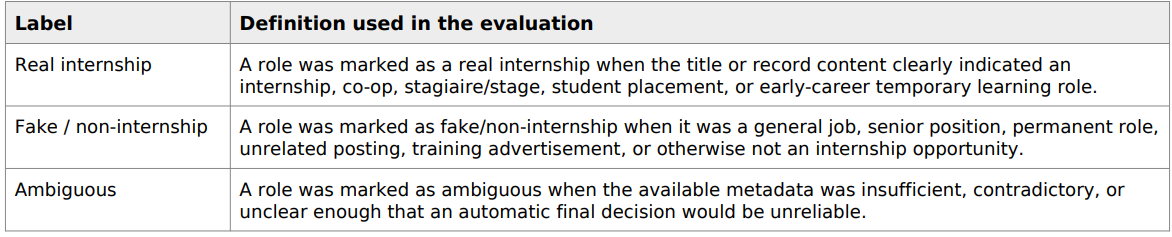
\includegraphics[width=\textwidth]{tables/appendices/Manual label definitions used in the evaluation.png}
\end{table}

\section{Human Inspection Sample Summary}
\label{appendix:human-inspection-summary}

\begin{table}[H]
    \centering
    \caption{Human inspection sample summary}
    \label{tab:frontend-catalog-statistics}
    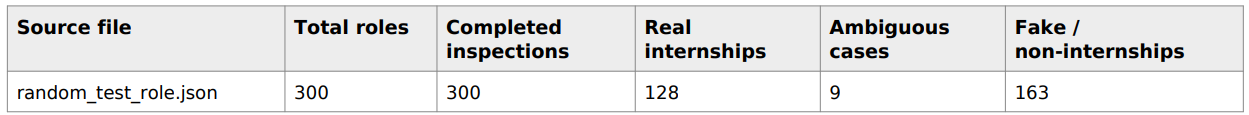
\includegraphics[width=\textwidth]{tables/appendices/Human inspection sample summary.png}
\end{table}

The manual sample confirms that scraped recruitment data contained a mixed set of valid
internships, non-internship roles, and borderline cases. This is the empirical basis for treating
internship discovery as a semantic filtering and uncertainty-management problem rather than a
simple keyword-search problem.

\section{Example Inspected Records}
\label{appendix:example-inspected-records}

\begin{table}[H]
    \centering
    \caption{Example inspected records}
    \label{tab:frontend-catalog-statistics}
    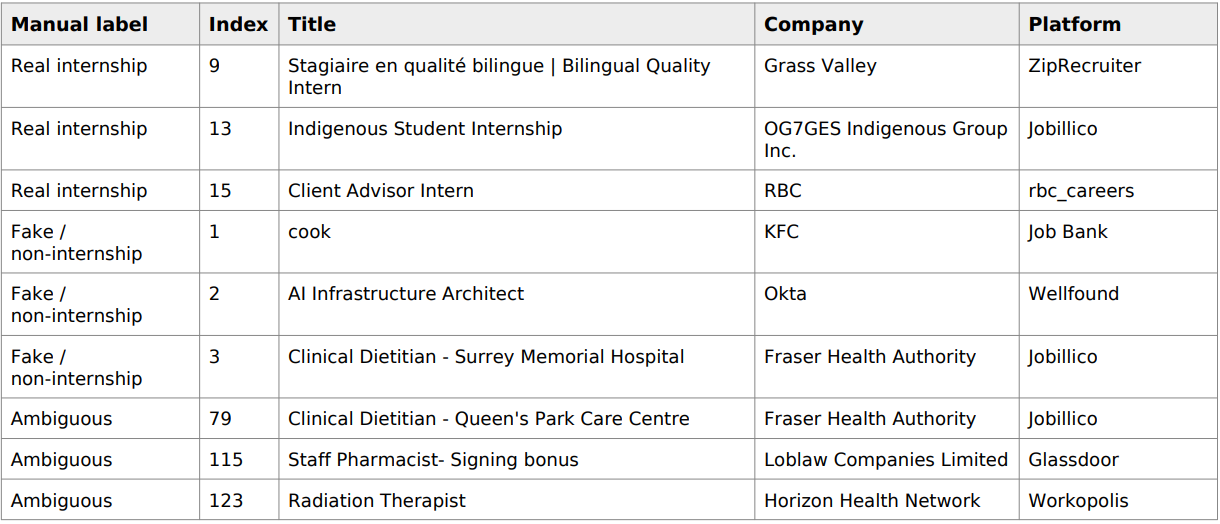
\includegraphics[width=\textwidth]{tables/appendices/Example inspected records.png}
\end{table}

\section{Files Supporting Appendix A}
\label{appendix:files-supporting-appendix-a}

\begin{table}[H]
    \centering
    \caption{Files supporting Appendix A}
    \label{tab:frontend-catalog-statistics}
    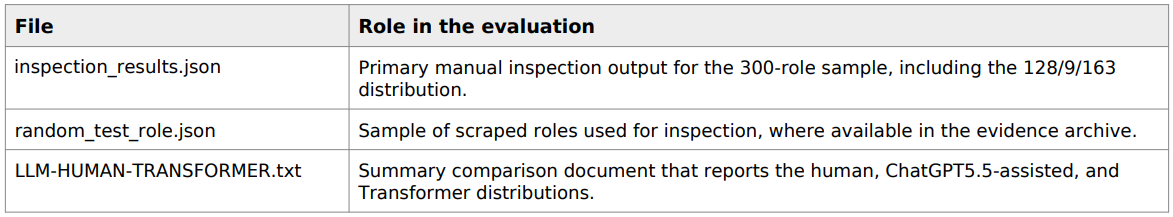
\includegraphics[width=\textwidth]{tables/appendices/Files supporting Appendix A.png}
\end{table}



\chapter{Internship Detection and Classification Evidence}
\label{appendix:classification-evidence}

This appendix supports the classification results discussed in Chapter 6. Human review is treated as
the reference for the inspected sample. ChatGPT5.5-assisted review is reported as sample-level
agreement with that reference, not as a claim of universal accuracy. The Transformer is evaluated
as a binary real/fake detector because it does not output an ambiguous class.

\section{Classification Comparison Table}
\label{appendix:classification-comparison-table}

\begin{table}[H]
    \centering
    \caption{Classification comparison table}
    \label{tab:frontend-catalog-statistics}
    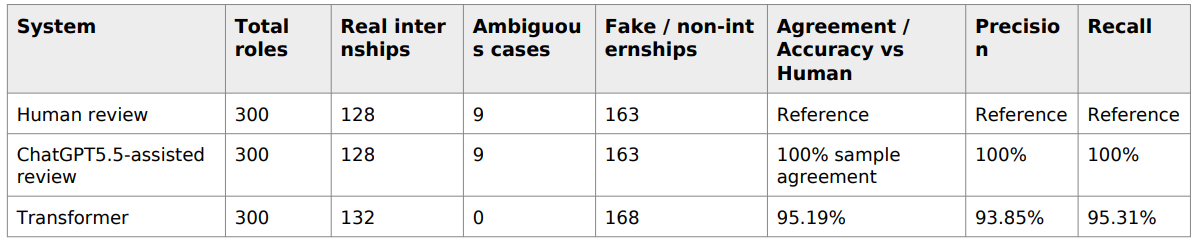
\includegraphics[width=\textwidth]{tables/appendices/Classification comparison table.png}
\end{table}

\section{Interpretation of the Metrics}
\label{appendix:interpretation-of-metrics}

Precision measures how trustworthy the system is when it classifies a role as a real internship. A
high precision score means that fewer fake or non-internship roles are incorrectly accepted as real
internships.

Recall measures how many real internships the system successfully finds. A high recall score
means that fewer genuine internships are missed.

The Transformer achieved 95.19\% accuracy, 93.85\% precision, and 95.31\% recall against the
human clear real/fake cases. Since the Transformer does not produce an ambiguous label,
ambiguous cases remain better handled through manual or ChatGPT5.5-assisted review. This
interpretation supports the uncertainty-management focus of the thesis.

\section{Classification Evidence Files}
\label{appendix:classification-evidence-files}

\begin{table}[H]
    \centering
    \caption{Classification evidence files}
    \label{tab:frontend-catalog-statistics}
    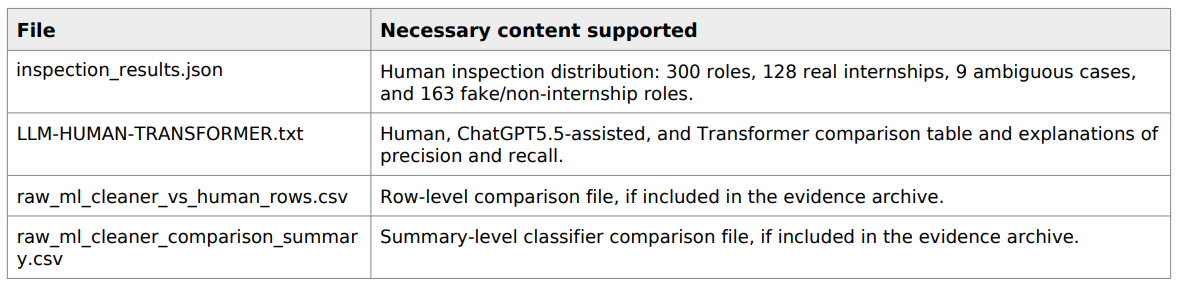
\includegraphics[width=\textwidth]{tables/appendices/Classification evidence files.png}
\end{table}

\chapter{Semantic Enrichment Rules, Vocabularies, and Pipeline Logic}
\label{appendix:semantic-enrichment-rules}

This appendix records the essential implementation logic behind the semantic enrichment pipeline
without reproducing the full codebase. It supports the claim that the pipeline combines
deterministic cleaning, rule-based internship signals, embedding-based classification, skill
extraction, domain categorization, deduplication, and manual-review indicators.

\section{Pipeline Flow}
\label{appendix:pipeline-flow}

\begin{itemize}
    \item Load raw JSON records from scraped or provided recruitment data.
    \item Normalize heterogeneous fields into a common internal representation.
    \item Remove invalid records and reduce noisy descriptions while preserving useful text structure.
    \item Deduplicate records using normalized links, title/company/location keys, and similarity checks.
    \item Apply transparent internship scoring rules using positive and negative role signals.
    \item Apply local Transformer/prototype classification when enabled and blend it with rule evidence.
    \item Extract controlled skills and classify a broad domain/category.
    \item Assign internship probability, final label, and manual-review indicators.
    \item Export accepted records into frontend-ready JSON for browsing, filtering, and inspection.
\end{itemize}

\section{Core Implementation Files}
\label{appendix:core-implementation-files}

\begin{table}[H]
    \centering
    \caption{Core implementation files}
    \label{tab:frontend-catalog-statistics}
    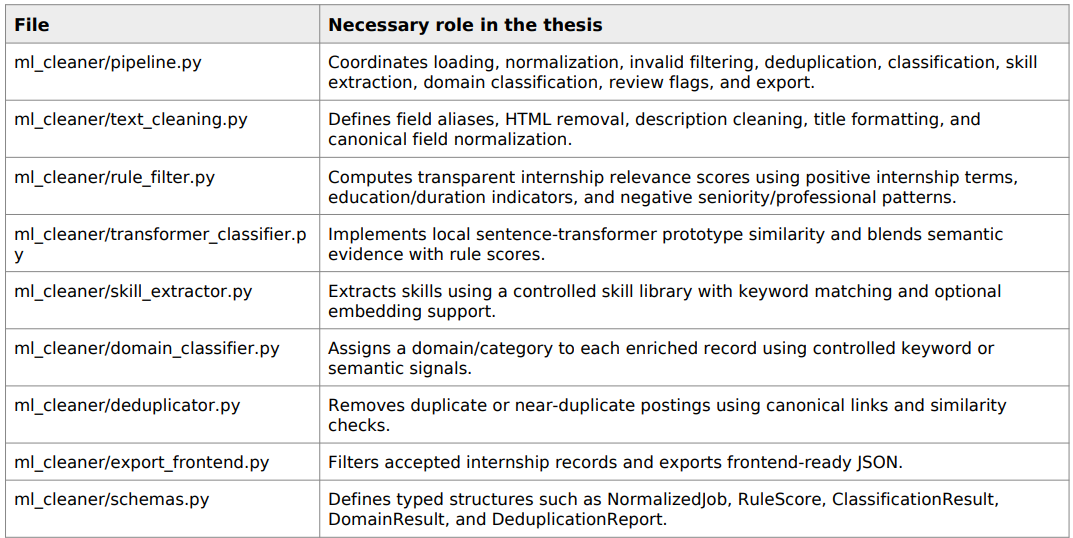
\includegraphics[width=\textwidth]{tables/appendices/Core implementation files.png}
\end{table}

\section{Configuration and Vocabulary Files}
\label{appendix:configuration-and-vocabulary-files}

\begin{table}[H]
    \centering
    \caption{Configuration and vocabulary files}
    \label{tab:frontend-catalog-statistics}
    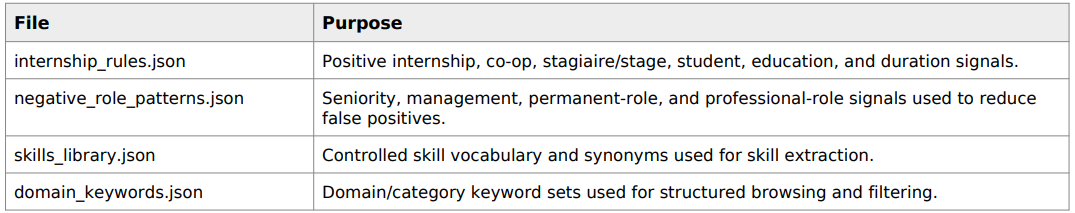
\includegraphics[width=\textwidth]{tables/appendices/Configuration and vocabulary files.png}
\end{table}

\section{Uncertainty and Manual-Review Logic}
\label{appendix:uncertainty-and-manual-review-logic}

The implementation does not force every uncertain posting into a confident final interpretation. The
manual-review indicator is triggered by uncertainty conditions such as probability falling inside a
review range, disagreement between rule and semantic evidence, weak semantic margin, or
conflict between an internship-looking title and a negative final decision. This supports RQ4 by
preserving ambiguity instead of hiding it behind a binary decision.

\begin{verbatim}
manual_review = (
    probability inside review range
    OR rule/semantic disagreement
    OR internship title conflicts with final decision
    OR semantic margin is weak
)
\end{verbatim}


\chapter{Structured Internship Schema and Frontend Catalog Evidence}
\label{appendix:structured-internship-schema}

This appendix shows the structured output expected from the enrichment pipeline and the
frontend-facing fields used for discovery. It supports RQ2 and RQ3 by connecting semantic
enrichment to concrete searchable and filterable record fields.

\section{Frontend-Ready Internship Record Schema}
\label{appendix:frontend-ready-schema}

\begin{table}[H]
    \centering
    \caption{Frontend-ready internship record schema}
    \label{tab:frontend-catalog-statistics}
    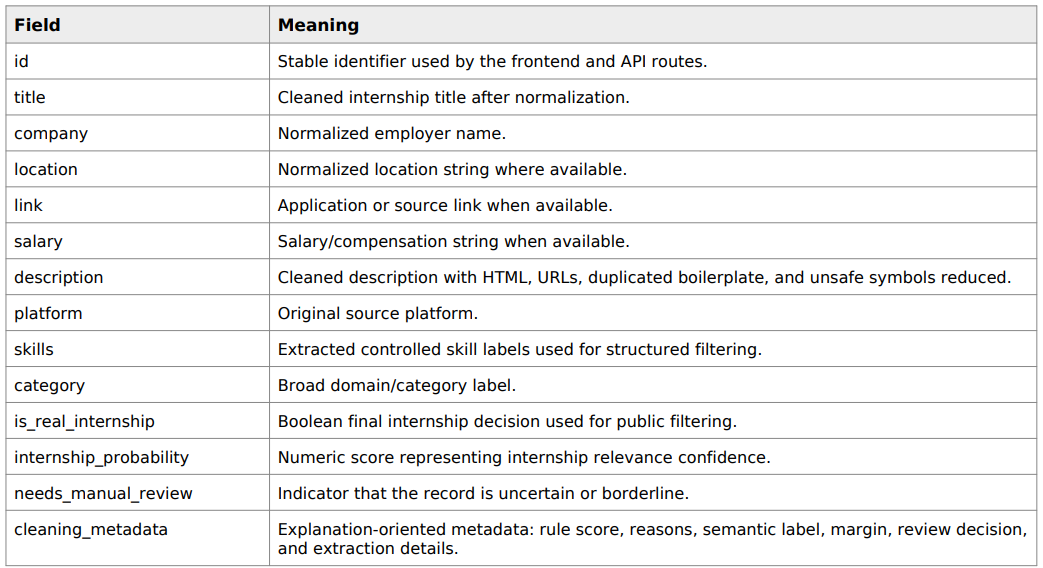
\includegraphics[width=\textwidth]{tables/appendices/Frontend-ready internship record schema.png}
\end{table}

\section{Enriched Catalog Statistics Used in Chapter 6}
\label{appendix:enriched-catalog-statistics}

\begin{table}[H]
    \centering
    \caption{Enriched catalog statistics used in Chapter 6}
    \label{tab:frontend-catalog-statistics}
    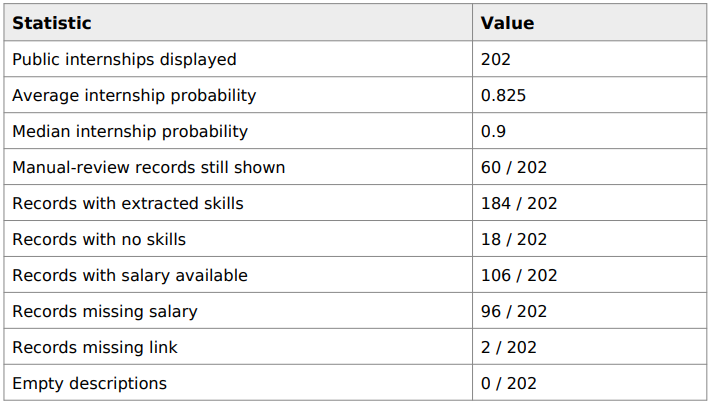
\includegraphics[width=\textwidth]{tables/appendices/Enriched catalog statistics used in Chapter 6.png}
\end{table}

\section{Example Structured Record Shape}
\label{appendix:example-structured-record-shape}

The following reduced example shows the record shape, not the full description text. It
demonstrates the fields that make the enriched catalog searchable, filterable, and reviewable.

\begin{verbatim}
{
  "id": "...",
  "title": "SAP IT Business Analyst Co-Op (Jan 2026)",
  "company": "Lockheed Martin Canada",
  "location": "Ontario",
  "skills": ["business", "education", "finance", "operations"],
  "category": "business",
  "is_real_internship": true,
  "internship_probability": 0.65,
  "needs_manual_review": true,
  "cleaning_metadata": {
    "rule_score": 0.55,
    "internship_label": "real internship",
    "semantic_label": "real internship",
    "semantic_margin": 0.0254
  }
}
\end{verbatim}

\section{Frontend Discovery Fields}
\label{appendix:frontend-discovery-fields}

Search and filtering are supported by enriched fields such as title, company, location, skills,
category, salary, description, internship probability, and review indicators. This supports structured
discovery without claiming formal user satisfaction or a completed user study.

\section{Files Supporting Appendix D}
\label{appendix:files-supporting-appendix-d}

\begin{table}[H]
    \centering
    \caption{Files supporting Appendix D}
    \label{tab:frontend-catalog-statistics}
    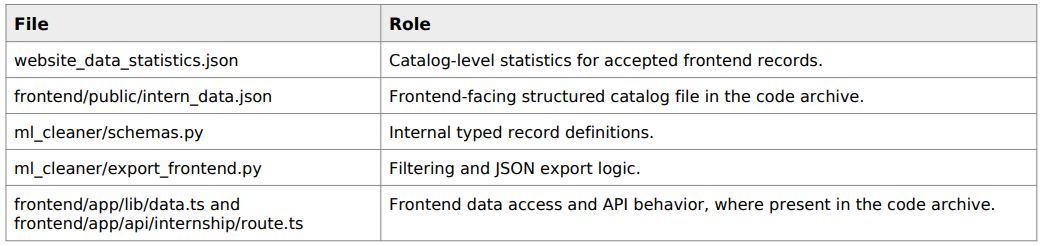
\includegraphics[width=\textwidth]{tables/appendices/Files supporting Appendix D.png}
\end{table}


\chapter{Evaluation Logs and Reproducibility Evidence}
\label{appendix:evaluation-logs-reproducibility}

This appendix lists the proof files needed to verify the operational and frontend-oriented
measurements used in Chapter 6. The logs are not pasted in full because the thesis should not
become a raw technical dump. The files should be kept in the evidence archive alongside the
thesis.

\section{Search and Filter Timing Evidence}
\label{appendix:search-filter-timing-evidence}

\begin{table}[H]
    \centering
    \caption{Search and filter timing evidence}
    \label{tab:frontend-catalog-statistics}
    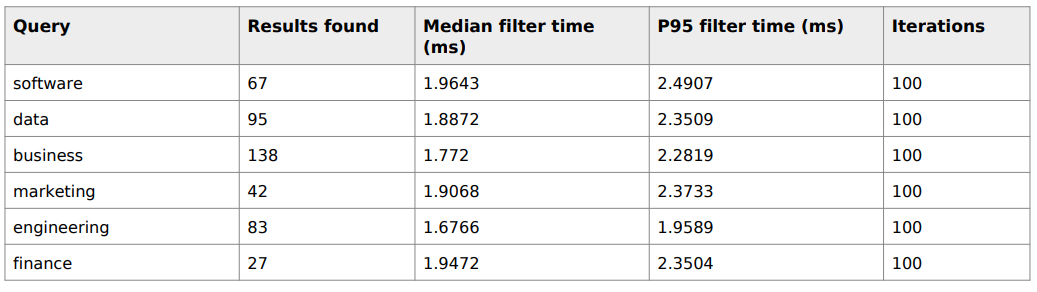
\includegraphics[width=\textwidth]{tables/appendices/Search and filter timing evidence.png}
\end{table}

\section{Local Frontend Response Evidence}
\label{appendix:local-frontend-response-evidence}

\begin{table}[H]
    \centering
    \caption{Local frontend response evidence}
    \label{tab:frontend-catalog-statistics}
    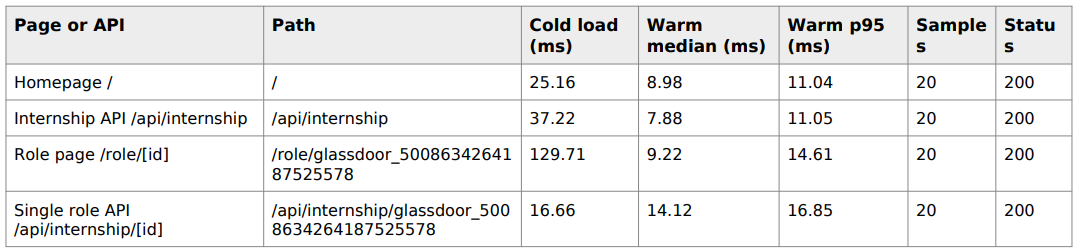
\includegraphics[width=\textwidth]{tables/appendices/Local frontend response evidence.png}
\end{table}

\section{Build and File-Size Evidence}
\label{appendix:build-and-file-size-evidence}

\begin{table}[H]
    \centering
    \caption{Build and file-size evidence}
    \label{tab:frontend-catalog-statistics}
    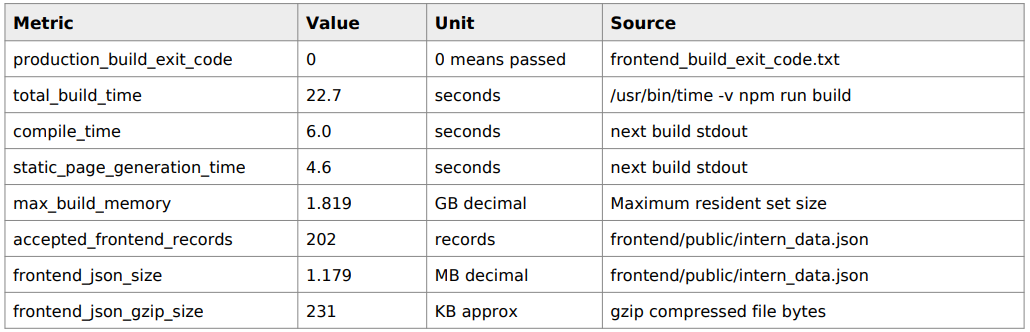
\includegraphics[width=\textwidth]{tables/appendices/Build and file-size evidence.png}
\end{table}

\section{Evidence Archive Index}
\label{appendix:evidence-archive-index}

\begin{table}[H]
    \centering
    \caption{Evidence archive index}
    \label{tab:frontend-catalog-statistics}
    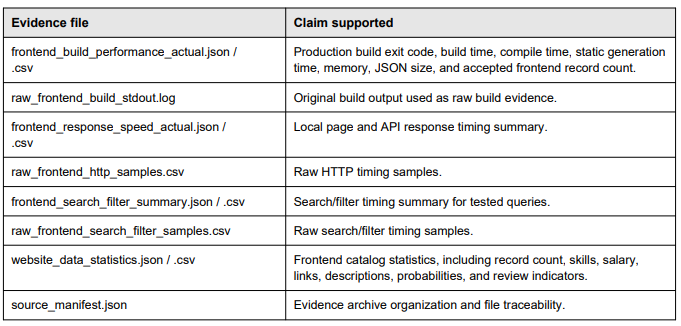
\includegraphics[width=\textwidth]{tables/appendices/Evidence archive index.png}
\end{table}

\section{Interpretation Boundary}
\label{appendix:interpretation-boundary}

These measurements should be described as local evaluation results observed under the tested
environment. They support local execution feasibility and structured discovery behavior, but they
do not prove universal cloud performance, production scalability, or user satisfaction. This
boundary is important for defending the research scope.



\end{document}
